\section{Overview}

In nature, most organic models ubiquitously contain cylindrical parts \cite{Zhou:2015:GCD}, e.g., arms, legs, etc. Moreover, an cylindrical part can be well represented by its corresponding 1{D} skeleton. Based on this property, a chunk of a mesh model can be fabricated free of support {if all the arcs of its corresponding skeleton piece subtend to a printing direction by an angle of no large than $\theta$.} Hence, our problem becomes partitioning a given 1{D} skeleton graph into a set of subgraphs such that each subgraph merits the desirable support-free property. In the remainder of the paper, by model we mean an organic mesh model of natural life form or articulated figures preserving nice topology features of real lives.

\textbf{Choise of skeleton.} Compared to natural skeletons, the medial axis can describe the topology of a mesh model more precisely \cite{ZhangXWYTW15}. However, a medial axis of a 3D mesh model is a 2D surface which cannot be conveniently applied to describe the critical topology changes of the model. Additionally, the medial axis consists of intersecting pieces of planes and conic surfaces, presenting significant complications to algorithms that attempt to construct 3D medial axes.
Reeb graph provides a possible choice for 1D skeleton. During the generation process of any reeb graph, the slicing direction and the position of the representative node on each slide (a connected region) seriously influence the choice of critical points and therefore generation of the Reeb graph. However, the determination of suitable slicing direction and representative nodes is an intractable problem. We resort to the 1D Laplacian skeleton proposed by \cite{AuTCCL08} which is extracted by shrinking the mesh model using Laplacian smoothing, such 1D Laplacian skeleton provides an excellent choice for reasonably describing the geometrical and topological variations of any 3{D} model.

%Figure \ref{fig:ex1} shows an example of the Laplacian skeleton.

%\begin{figure}[tbp]
%  \centering
% \mbox{} \hfill
%\includegraphics[width=0.4\textwidth]{figs/tree_with_skeleton.png}
%\caption{\label{fig:ex1}%
%        An illustration of a 3D mesh model and its 1D Laplacian skeleton. }
%\end{figure}



\textbf{Problem Statement.} Our goal is hence to decompose the 1D Laplacian skeleton of the model into {{a proper number of support-free subgraphs leads to a partition of the model into the least printable parts free of support structures and seams on the final assembled model.}} In addition, since support structures result in bumpy supported areas, support-free fabrication also means a nice preservation of the surface quality of the parts. Further, a minimization of the number of cuts and the total cutting length means a minimum amount of seams and their lengths on the assembled model. Therefore, we focus on these two problems in this paper.

{\color{red}{Finding a decomposition of the skeleton into the least pieces of support free subgraphs is a non-trivial task. As a simple example, {{suppose for simplicity that the least number of cuts on the skeleton corresponds to the least number of cuts on the mesh model}}, refer to Figure \ref{fig:fork}, consider a 1{D} Laplacian skeleton that is a fork with $n$ arcs sharing a common origin; consider partitioning the fork into the least number of sub-forks such that each sub-fork can be packed into a cone of angle $2\theta$ in order to make the sub-fork support-free when fabricated in a given direction, where $\theta$ is defined based on the printing experiments as a safe angle allowing support-free fabrication.

\emph{\textbf{Lemma 1}: Partitioning a graph into the least number of support-free subgraphs is NP-hard.}

\emph{Proof}:  
We shall complete the proof by transforming an instance of a known $NP$ hard problem into our problem in polynomial time.
First we need to show that our problem is in $NP$: The certificate is a set of arc-disjoint and rooted subgraphs of the skeleton graph, a certifier checks in polynomial time (i.e., $O(n^2)$) that the size of the set is at most the given bound $K$, and that the rooted subgraphs satisfy the angle constraint of $2\theta$.
We shall reduce the clique cover problem to the skeleton partition problem, i.e., where the clique cover problem is covering a graph with the least number of cliques (complete graphs), which has been shown to be $NP$-hard [Karp]. We now show that Clique Cover ��$p$ Skeleton Partition. We define the following instance of Clique Cover: an arbitrary planar $G(V, E)$ such that $|V| = n$ and each pair of nodes ($v_i$, $v_j$) is connected by an arc $|v_iv_j|$ is no larger than a given bound $D$. Construct a skeleton $S$ of $n$ arcs rooted at a common node as follows: select any triplet of nodes {$v_i$, $v_j$, $v_k$} from $G$ and construct a triplet of unit arcs $\{e_i, e_j, e_k\}$ in $S$, the angle between each pair of arcs $\{e_i, e_j\}$, denoted as $A(e_i, e_j)$, is defined as $A(e_i, e_j) = 2|v_iv_j|/D$. See Figure \ref{fig:fork}, given this triplet of arcs as the basis (three distinct vectors in 3{D} space), we can construct each of the remaining arcs of $S$, denoted as $e_x$, which represents a node $v_x$ in $G$: the relative position of $e_x$ with respect to each element of $\{e_i, e_j, e_k\}$ is defined as the relative distance from $v_x$ with respect to each element of $\{v_i, v_j, v_k\}$. This transformation takes $O(n^2)$ time.



\begin{figure}[t!]
  \centering
  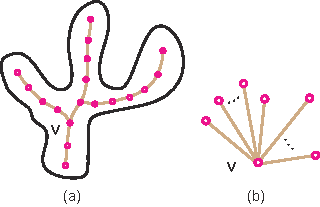
\includegraphics[width=0.6\linewidth]{figs/fork.png}
  \caption{\label{fig:fork}%
           A skeleton $S$ that is a fork originated from a node.}
\end{figure}

Now we claim that there is a clique cover in $G$ of size $K$ if and only if there is a skeleton partition of $S$ into $K$ subgraphs with the angle constraint, i.e., the angle between each pair of arcs in a subgraph is no larger than $2\theta$.
For if there is clique cover in $G$ of size $K$, then each clique in $G$ corresponds to a rooted subgraph of $S$ satisfying the angle constraint. Conversely, if $S$ is partitioned into $K$ subgraphs satisfying the angle constraint, then all pairs of arcs in each rooted subgraph satisfy the angle constraint, by the mapping relation, their corresponding nodes in $G$ form a clique. This completes the proof. \qed

This tells the difficulty of solving the problem of partitioning a 3D model into the least number of support free pieces. In the following, we shall show how to solve the problem with a practical yet efficient algorithm.}}

We formulate the partition problem with the objectives of both the total number of cuts and the cutting length, under the constraint of printing angle of each branch with respect to the build platform, the angle between a cutting plane and the printing direction, the dimension of each printed model with respect to the printable volume of a given printer, and the base area of a printed model. Since the problem is NP-hard, we propose a randomized Monte Carlo method in compliance with a set of carefully designed selection strategy to seek a practical solution. Figure \ref{fig:ex1} shows an example of a deer model (shell), our partition result based on Laplacian skeleton of the model, the printing result and the assembly effect. The details of Mento Carlo method is given below.


